\documentclass[11pt]{beamer}
\usepackage{helvet} %font
\beamertemplatenavigationsymbolsempty
\usetheme{JuanLesPins}
\usefonttheme{structurebold}

\usepackage[french]{babel}
\usepackage[utf8]{inputenc}
\usepackage[T1]{fontenc}
\usepackage{amssymb,amsmath}
\usepackage{tikz}
\usepackage{geometry}
\usepackage{xcolor,colortbl}
\usetikzlibrary{arrows,positioning}
\usepackage{listings}

\AtBeginSubsection[]
{
   \begin{frame}
	\small \tableofcontents[currentsection]
   \end{frame}
}

\newenvironment{slide}[1]{%
\begin{frame}[environment=slide]
\frametitle{#1}
}{%
\end{frame}
}
\setbeamercolor{structure}{fg=red}
\setbeamercolor{frametitle}{bg=black,fg=white}
\definecolor{gris}{gray}{0.6}
\definecolor{grisclair}{gray}{0.9}

\newtheorem{exercice}{Exercice}

\title{Machine Learning VIII : Minimisation du risque}
\author{Nicolas Bourgeois}
\date{}

\newcommand{\Python}[1]{
	{\small	\lstinputlisting[language=Python]{./#1.py}}
}
\newenvironment{pyenvsmall}
	{ \ttfamily \tiny }
	{\par  }

\newcommand{\Pythonsmall}[1]{
	{\scriptsize \lstinputlisting[language=Python]{./#1.py}}
}
\newcommand{\elimine}[1]{{\textcolor{lightgray}{#1}}}

\newcommand\Wider[2][3em]{%
\makebox[\linewidth][c]{%
  \begin{minipage}{\dimexpr\textwidth+#1\relax}
  \raggedright#2
  \end{minipage}%
  }%
}

\begin{document}

\begin{frame}
\maketitle
\end{frame}

\begin{frame}
\tableofcontents
\end{frame}


\section{Outils de base}

\subsection{Loss Function}

\begin{frame}{Principe}
Soit $LF:E \rightarrow \mathbb{R}_+$ une fonction de perte, telle que
$$LF(Y,Y) = 0$$\\
Et $\Phi$ une fonction d'agrégation

Objectif :
$$ \min_f \Phi_{i \in I} \left( LF(f(X_i),Y_i) \right)$$

\end{frame}

\begin{frame}{Exercice}
\begin{exercice}
Suggérez des fonctions de perte pour la régression
\end{exercice}

\vspace{0.3cm}

\begin{exercice}
Suggérez des fonctions de perte pour la classification
\end{exercice}
\end{frame}

\begin{frame}{Solution}
1)\\
$LF(X,Y) = (X-Y)^q$\\
$LF(X,Y) = \frac{|X-Y|}{|X+Y|}$\\
\vspace{0.3cm}
2)\\

$LF(X,Y) = \mathbf{1}_{X\neq Y}$\\
$LF(X,Y) = 1$ si $X>Y$, $\epsilon$ si $X<Y$, $0$ sinon.  

\end{frame}

\begin{frame}{Exercice}
\begin{exercice}
En reprenant les données iris, programmez (sans utiliser scipy ou scikit-learn) une régression linéaire entre la longueur et l'épaisseur des pétales, en choisissant respectivement :
\begin{itemize}
	\item $LF(X,Y) = (X-Y)^2$
	\item $LF(X,Y) = |X-Y|$
\end{itemize}
Affichez les deux droites sur le même graphe.
\end{exercice}

\end{frame}

\begin{frame}{Résultat attendu}
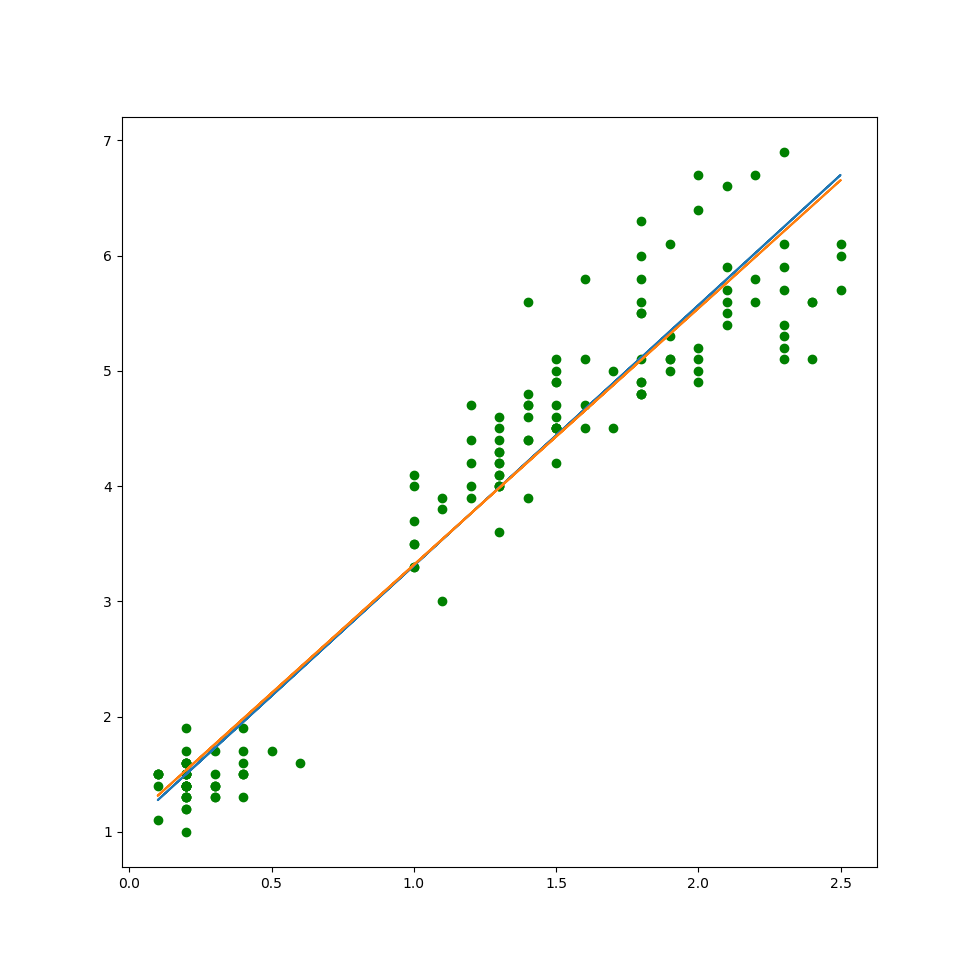
\includegraphics[scale=0.4]{ext1}
\end{frame}

\begin{frame}{Solution}
\Python{ext1.py}
\end{frame}

\subsection{Risque empirique}

\begin{frame}{Principe}

\end{frame}

\begin{frame}{Exercice}

\end{frame}

\begin{frame}{Solution}

\end{frame}

\subsection{Matrice de confusion}

\begin{frame}{Principe}

\end{frame}

\begin{frame}{Exercice}

\end{frame}

\begin{frame}{Solution}

\end{frame}

\subsection{Scatter Plot}

\begin{frame}{Principe}

\end{frame}

\begin{frame}{Exercice}

\end{frame}

\begin{frame}{Solution}

\end{frame}

\section{Risque et Consistance}

\begin{frame}{Principe}

\end{frame}

\begin{frame}{Exercice}

\end{frame}

\begin{frame}{Solution}

\end{frame}

\subsection{Motivation}

\begin{frame}{Principe}

\end{frame}

\subsection{Risque}

\begin{frame}{Principe}

\end{frame}

\begin{frame}{Exercice}

\end{frame}

\begin{frame}{Solution}

\end{frame}

\subsection{Consistance}

\begin{frame}{Principe}

\end{frame}

\begin{frame}{Exercice}

\end{frame}

\begin{frame}{Solution}

\end{frame}

\section{Empirical Risk Minimization}

\begin{frame}{Principe}

\end{frame}

\begin{frame}{Exercice}

\end{frame}

\begin{frame}{Solution}

\end{frame}

\subsection{ERM}

\begin{frame}{Principe}

\end{frame}

\begin{frame}{Exercice}

\end{frame}

\begin{frame}{Solution}

\end{frame}

\subsection{exemples}

\begin{frame}{Principe}

\end{frame}

\begin{frame}{Exercice}

\end{frame}

\begin{frame}{Solution}

\end{frame}

\subsection{généralisation}

\begin{frame}{Principe}

\end{frame}

\begin{frame}{Exercice}

\end{frame}

\begin{frame}{Solution}

\end{frame}

\end{document}